% This is LLNCS.DOC the documentation file of
% the LaTeX2e class from Springer-Verlag
% for Lecture Notes in Computer Science, version 2.4
\documentclass{llncs}
\usepackage{llncsdoc}
\usepackage{graphicx, caption, subcaption}
\usepackage{todonotes}
\usepackage{float}
\usepackage{booktabs}
\usepackage{graphicx}
\usepackage{amsmath}
\usepackage{hyperref}
\usepackage{amssymb}
\renewcommand{\arraystretch}{1.2}
\DeclareMathOperator*{\argmax}{argmax}
\DeclareMathOperator*{\avg}{average}

\begin{document}

\newpage

\title{Playing Ludo with Artificial Intelligence}
\author{Mathias Emil Slettemark-Nielsen}
\institute{University of Southern Denmark, Campusvej 55, 5230 Odense M, Denmark \\masle16@student.sdu.dk}
\maketitle

\begin{abstract}
This paper demonstrates methods for making an intelligent Ludo playing agent. Three different methods are implemented that are based on Artificial Neural Networks. The parameters of the methods are found by the use of Evolutionary Algorithms, which optimize the parameters based on the "Survival of the fittest". Different Evolutionary Algorithms methods were used for the optimization of Artificial Neural Networks. The final developed player has a win rate of $92.5\ \%$ against a random player.
\end{abstract}

\section{Introduction} \label{sec:intro}
Ludo has always been an unpredictable game and most of the time, no matter how hard you try, winning the game mostly relies on luck. However, this will be no more because of Artificial Intelligence which allows for the creation of autonomous players/agents.

More specific with the use of Evolutionary Algorithms, EA, that makes the creation of agents less comprehensive. Throughout this paper multiple Ludo players will be evolved with EA, and evaluated versus random and handcrafted players.

The Ludo game used in this report is a python version of the provided c++ version that can be found at \cite{ludo_game}. Python is used instead of c++ for faster development.

The implementation of this report can be found at \url{https://github.com/Masle16/ludo_ai2}.

\section{Methods} \label{sec:methods}
The ludo game consist of a discrete set of environment states $s$ and a discrete set of agent actions $a$. $s$ is the position of all the tokens, even though there are many different combinations of how the tokens can be placed it is still a finite state problem. $a$ is to choose between the four tokens. The state representation of the ludo game contains the current state and the next states based on the dice roll. The current state is the position of all the tokens, and the next state is the position of all the tokens after a certain token is moved.

The agents policy $\pi$ specifies what $a$ to choose in any $s$. To find the best $a$ a value function $V$ is introduced that estimates a relative score of a state. To find the optimal $V$, value iteration is used. The $\pi$ is then to choose the action which maximizes $V$ by
\begin{equation}
\label{eqn:policy}
\pi(s) = \argmax_a \sum_{s'} P(s' | s,a) V(s'(s,a))
\end{equation}
where $P$ is the probability of the next state $s'$ given $s$ and $a$. In ludo the immediate state transition is deterministic, thus equation \ref{eqn:policy} yields
\begin{equation}
\label{eqn:ludo_policy}
\pi(s) = \argmax_a V (s'(s,a))
\end{equation}
where $s'$ is the immediate next state after an $a$, and $V$ depends on the agents chromosome $\theta$ and action representation $A$. Equation \ref{eqn:ludo_policy} then becomes
\begin{equation}
\label{eqn:value_function}
\pi(s) = \argmax_a V(\theta, A(s, s'(s,a)))
\end{equation}

In this paper different action representations are developed and will be elaborated in section \ref{subsec:action_representaion}. To find the optimal chromosome, the general scheme of an EA from \cite{ec:springer} is used and will be elaborated in section \ref{subsec:ea}.

\subsection{Action Representation of a Ludo Game} \label{subsec:action_representaion}
The value function $V$ from equation \ref{eqn:value_function} denotes how good a move with a specific token is, therefore to win a ludo game the token that enlarges the players winning opportunity must be moved. The value function depends on the chromosome, described in section \ref{subsec:ea} and action representation of the ludo game.

Many different action representations can be made with and without domain knowledge, where the state can include all the positions of the tokens or be represented by a binary format where each index contains true or false about the tokens condition.
% Many different action representations can be made, e.g. a state can include the position of all tokens or a tokens state could be represented by a binary format where each index contains true or false about the tokens condition.

In this paper one action representation with domain knowledge of the ludo game and two without are implemented.

\textbf{Simple:} A simple action representation, $A_{simple}$, is developed with $4$ binary components. 1: The token is moved out of home, 2: The token enters the winner road, 3: The token enters goal and 4: The token sends a opponent token home. The value function for one token is
\begin{equation}
V_{simple}(\theta, A_{simple}) = \sum_{i=1}^{4} \theta_{i} A_{simple, i}
\label{eqn:value_simple}
\end{equation}
and a policy is the found as in equation \ref{eqn:value_function}. The chromosome is normalized when it is changed by the EA, thus the $\sum_i |\theta_i| = 4$. The $A_{simple}$ calculates the relative score of a state based on the current state and immediate next state.

The simple action representation requires domain knowledge, i.e. that the developer knows the important aspects of a ludo game. However, the things that a human finds important to win a ludo game might not be the case. Therefore, is an artificial neural network approach implemented where the immediate next state based on a token move is passed as input, and the current state is not used.

\textbf{Advanced:} The advanced action representation uses a small artificial neural network with $4 \cdot 59 = 236$ input neurons, $4$ hidden neurons and $1$ output neuron. The number of hidden neurons is chosen based on the simple action representation which uses a chromosome with a length of $4$ to pick a token. The input is the next state for a token move, thus a value is estimated for each tokens next state and the token with the highest value is moved. Both the hidden and the output neurons use Tanh that outputs a number between $-1$ and $1$. The network consist of $(4 \cdot 59) \cdot 4 + 4 \cdot 1 = 948$ parameters or genes.

The advanced action representation is somewhat a small network, therefore a larger network is also implemented.

\textbf{Full:} The full player resembles the advanced player, however, a bias is added to the input, and $100$ hidden neurons is used. The network structure of the full action representation is then $4 \cdot 59 + 1 = 237$ input neurons, $100$ hidden neurons and $1$ output neuron. The input is the same as in the advanced method and Tanh is also used as the activation function for both hidden and output neurons. The network consist of $(4 \cdot 59 + 1) \cdot 100 + 100 \cdot 1 = 23800$ parameters or genes. The bias term will be explained in section \ref{subsec:weight_init}.

Note that the advanced and full action representation estimates the relative score of an immediate next state based on only the immediate next state and not the current state.

The three action representations will be denoted as players throughout the report, e.g. the simple player.

\subsection{Components of Evolutionary Algorithms} \label{subsec:ea}
To find the optimal weights for the chromosome for each player from section \ref{subsec:action_representaion} EA is used. EA aims at approximating the optimal weights for the players based on the "Survival of the fittest".

Real values are used as the gene values in the chromosomes, i.e. the gene values come from a continuous distribution, as suggested in \cite{ec:springer} when evolving weights on the connections between the neurons in an artificial neural network. The chromosome with $k$ genes is then a vector $\langle x_1, \dots, x_k \rangle$ with $x_i \in \mathbb{R}$.

EA consist of $4$ main parts: evaluation, selection, reproduction, and replacement, and there are many different ways of doing each part. Thus, for each part the explored components of EA from \cite{ec:springer} will be elaborated.

\textbf{Evaluation:} The agents are evaluated by playing against each other in a tournament instead of playing against a fixed opponent, e.g. a random player. Thereby, fewer games are required and the agent will not just be good against a fixed opponent but it will learn its vulnerabilities, ideally making it more robust.

\textbf{Selection:} Tournament selection is used, thus $4$ chromosomes from the population play $N$ games against each other and the agents with most wins are selected for reproduction. A generation is defined to be when all chromosomes have played in a tournament. This is denoted as \textit{normal} selection and a player evolved with normal selection will be referred to as \texttt{s:Normal - population size - games per tournament}. Furthermore, cellular and island selection are explored in this paper. In \textit{cellular} selection, the population is split into a number of overlapping subpopulations by distributing the population on a grid with one chromosome per node, thus creating a neighborhood. The evaluation, selection, reproduction, and replacement is performed for each neighborhood. A player evolved with cellular selection will be denoted \texttt{s:Cellular - population size - games per tournament}. In \textit{island} selection, multiple populations are evolved on their island and after a number of generations, a number of chromosomes are selected from each island to be exchanged with others. A player evolved with island selection will be denoted \texttt{s:Island - island count - chromosome per island - generation per selection - migration count - games per tournament}.

\textbf{Reproduction:} Firstly, the two selected parents chromosomes $x$ and $y$ are recombined into offspring $z$. To create new offspring $\alpha$ is introduced, that creates a new gene value by $z_i = \alpha x_i + (1-\alpha) y_i$. In this paper three recombination types are explored: uniform, whole, and blend. In \textit{uniform} arithmetic recombination each gene from either parent is chosen with equal probability. A player evolved with uniform recombination will be denoted \texttt{r:Uniform}. In \textit{whole} arithmetic recombination the child gene is the weighted sum of the two parents gene. A player evolved with whole recombination will be denoted \texttt{r:Whole}. In \textit{blend} crossover a child is created by sampling a random number $u$ and calculating $\gamma = (1 - 2 \alpha)u - \alpha$, the new gene is then $z_i = (1-\gamma) x_i + \gamma y_i$. From \cite{ec:springer} the best results of blend crossover were found with $\alpha=0.5$ and will be used throughout this paper. Thus, the values are equally likely to lie inside the two parent's values as outside, thereby balancing exploration and exploitation. A player evolved with Blend recombination will be denoted \texttt{r:Blend - alpha}.

Secondly, mutation is applied to the offspring to maintain genetic diversity. The mutation methods normal, OneStep, and NStep from \cite{ec:springer} are explored. The \textit{normal} mutation changes the chromosomes by adding a value drawn randomly from a normal distribution with mean zero and specified standard deviation, $\sigma$, to each gene value. A player evolved with normal mutation will be denoted \texttt{m:Normal - sigma}. The \textit{OneStep} mutation stores the $\sigma$ within the chromosome, thus allowing the EA to find a good $\sigma$ itself. A player evolved with OneStep mutation will be denoted \texttt{m:OneStep}. The \textit{NStep} stores a $\sigma$ per gene within the chromosome, thus allowing the EA to adjust the $\sigma$ to the corresponding gene. A player evolved with NStep mutation will be denoted \texttt{m:NStep}.

\textbf{Replacement:} The final step is to replace bad chromosomes of the current generation with mutated offspring of the good chromosomes for the new generation. The two chromosomes with the lowest win rate after a tournament are replaced by the new mutated offspring. When the replacement has been performed EA will start a new generation at the evaluation step.

When denoting the EA combinations of a player, \texttt{s} is used for selection, \texttt{r} for recombination and \texttt{m} for mutation, e.g. a player evolved with normal selection with a population size of $20$ and $10$ games per tournament, Blend recombination with $\alpha=0.5$ and normal mutation with $\sigma=0.1$ is written as \texttt{s:Normal-20-10 r:Blend-0.5 m:Normal-0.1}.

In this paper, the genes in the chromosomes are sampled from a normal distribution, the learning rate of OneStep and NStep is set to $0.01$ and the $\sigma$ for mutation is sampled from a lognormal distribution as suggested in \cite{ec:springer}.

The best performing chromosome within the final population is found by recursively choosing the best chromosome from the population. For each recursion, elimination tournaments are played with $2500$ games per tournament, the best from each tournament pass on to the next recursion until the best chromosome is left. If not four chromosomes are available random players are inserted until a ludo game can be played.

\subsection{Players used in this Paper}
The standard opponents for the evaluation of the developed players are explained in this section.

\textbf{Random:} The random player simply takes a random action among the action of which it can take.

\textbf{Smart:} The smart player tries to move tokens out of home, otherwise, it moves the token which minimizes the player positions compared to the opponent's positions.

\textbf{Fellow-student:} The fellow-student method \cite{mikkel} is a Q-learning player where the agent creates a Q-table of all states it can be situated in, and all the actions it can take in that specific state. For each action in that specific state, a Q-value is attached and the agent will choose the action which produces the highest Q-value. The fellow-student player has a simplified action representation with five actions. 1: move out of spawn, 2: move into the goal, 3: send opponent home, 4: send self home and 5: move token.

\section{Results} \label{sec:results}
When comparing two players against each other two instances of each player are created, thereby making it a two versus two match. Furthermore, $2500$ games are played when comparing which gives a worst case standard deviation of $\sigma = \sqrt{0.5(1-0.5)/2500}=0.01$. In all tournaments the players order are randomly shuffled at every game. The comparison of players can be seen in table \ref{tab:player_eval}.

\begin{table}[]
\centering
\resizebox{\textwidth}{!}{%
\begin{tabular}{@{}l|cc|ccc|c@{}}
\toprule
\textbf{Player \textbackslash Opponent} & \textbf{Random} & \textbf{Smart} & \textbf{Simple} & \textbf{Advanced} & \textbf{Full} & \textbf{Fellow-student} \\ \midrule
\textbf{Random} & 50.9* & 17.1 & 18.5 & 8.9 & 7.2 & 26.8 \\
\textbf{Smart} & 83.8 & 49.5* & 54.7 & 38.5 & 31.8 & 66.2 \\ \hline
\textbf{Simple} & 80.1 & 44.0 & 50.5* & 29.0 & 24.9 & 57.2 \\
\textbf{Advanced} & 91.6 & 61.9 & 71.3 & 49.0* & 44.0 & 80.6 \\
\textbf{Full} & \textbf{92.5} & \textbf{68.6} & \textbf{74.0} & \textbf{56.9} & \textbf{50.2}* & \textbf{82.6} \\ \hline
\textbf{Fellow-student} & 72.6 & 32.6 & 42.7 & 20.6 & 15.8 & 50.2* \\ \bottomrule
\end{tabular}%
}
\caption{Win rate \% of two players vs. two opponents for $2500$ games. *Results that are statistical insignificant with a confidence level of $95\ \%$.}
\label{tab:player_eval}
\end{table}

\section{Analysis and Discussion} \label{sec:discussion}
Firstly, a statistical perspective of the results will be explained. Secondly, the evolution of the players and their results will be discussed. Lastly, some thoughts for improvement will be stated.

\subsection{Statistical Significance of Results}
A ludo player can either win or lose, which is a binary random variable with a true mean $\mu$ that also denotes the win rate. A binomial z test \cite{z_test} is performed on the win rates in table \ref{tab:player_eval}, where the statistical insignificant is marked with a '*'. The null hypothesis of the z test is that $\mu = 0.5$ and the critical value with a $95\ \%$ critical region is $\pm 1.6449$. 

\subsection{Evolution of the Simple Player}
To find a good chromosome for the simple player different EA combinations are explored. This is done by first investigating the different recombination methods, then different mutation methods, and then evaluating the most promising.

\textbf{Recombination methods:} Figure \ref{fig:recombination_method_simple} shows the genes of the simple player during the evolution process of different recombination methods with a population size of $100$ and $10$ games per tournament. Furthermore, normal selection and no mutation is used.
\begin{figure}[t]
    \centering
    \begin{subfigure}[t]{0.24\textwidth}
        \centering
        \captionsetup{width=.9\textwidth}
        \includegraphics[width=\textwidth]{figures/recombination/simple_normal-100-10_0-1.png}
        \caption{None.}
        \label{subfig:recomb_none_01}
    \end{subfigure}
    \begin{subfigure}[t]{0.24\textwidth}
        \centering
        \captionsetup{width=.9\textwidth}
        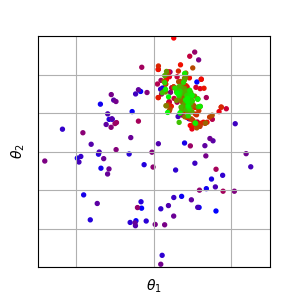
\includegraphics[width=\textwidth]{figures/recombination/simple_normal-100-10_uniform_0-1.png}
        \caption{Uniform.}
        \label{subfig:recomb_uniform_01}
    \end{subfigure}
    \begin{subfigure}[t]{0.24\textwidth}
        \centering
        \captionsetup{width=.9\textwidth}
        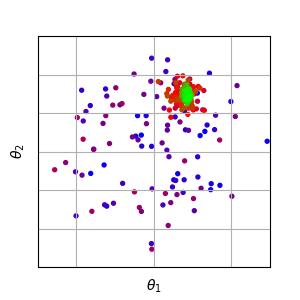
\includegraphics[width=\textwidth]{figures/recombination/simple_normal-100-10_whole_0-1.png}
        \caption{Whole.}
        \label{subfig:recomb_whole_01}
    \end{subfigure}
    \begin{subfigure}[t]{0.24\textwidth}
        \centering
        \captionsetup{width=.9\textwidth}
        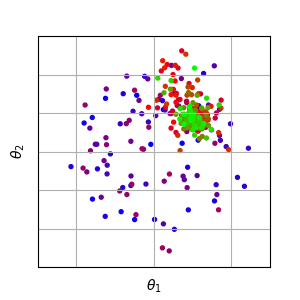
\includegraphics[width=\textwidth]{figures/recombination/simple_normal-100-10_blend-0.5_0-1.png}
        \caption{Blend with $\alpha=0.5$.}
        \label{subfig:recomb_blend_01}
    \end{subfigure}
    
    \begin{subfigure}[t]{0.24\textwidth}
        \centering
        \captionsetup{width=.9\textwidth}
        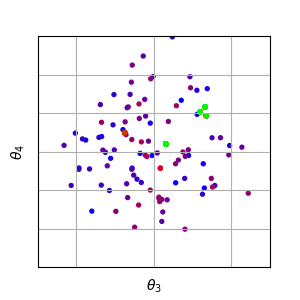
\includegraphics[width=\textwidth]{figures/recombination/simple_normal-100-10_2-3.png}
        \caption{None.}
        \label{subfig:recomb_none_23}
    \end{subfigure}
    \begin{subfigure}[t]{0.24\textwidth}
        \centering
        \captionsetup{width=.9\textwidth}
        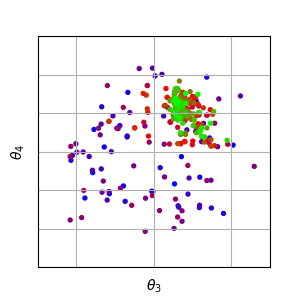
\includegraphics[width=\textwidth]{figures/recombination/simple_normal-100-10_uniform_2-3.png}
        \caption{Uniform.}
        \label{subfig:recomb_uniform_23}
    \end{subfigure}
    \begin{subfigure}[t]{0.24\textwidth}
        \centering
        \captionsetup{width=.9\textwidth}
        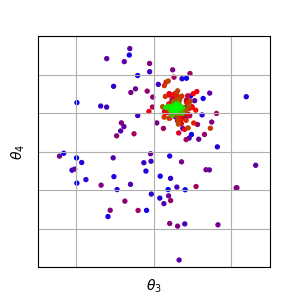
\includegraphics[width=\textwidth]{figures/recombination/simple_normal-100-10_whole_2-3.png}
        \caption{Whole.}
        \label{subfig:recomb_whole_23}
    \end{subfigure}
    \begin{subfigure}[t]{0.24\textwidth}
        \centering
        \captionsetup{width=.9\textwidth}
        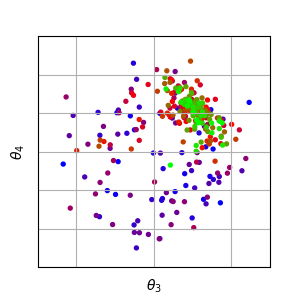
\includegraphics[width=\textwidth]{figures/recombination/simple_normal-100-10_blend-0.5_2-3.png}
        \caption{Blend with $\alpha=0.5$.}
        \label{subfig:recomb_blend_23}
    \end{subfigure}
    \caption{Evolution of the simple player with a population size of $100$ and $10$ games per tournament for $20$ generations with different recombination methods. The color range of the plots goes from blue to green, thus a green area indicate many chromosomes.}
    \label{fig:recombination_method_simple}
\end{figure}
From figures \ref{subfig:recomb_none_01} and \ref{subfig:recomb_none_23} it can be seen that the none recombination method does not explore the entire space, this is of course expected. However, notice in figures \ref{subfig:recomb_uniform_01} and \ref{subfig:recomb_uniform_23} the space is more explored but centered in the top half of the plot. The recombination method whole shown in figures \ref{subfig:recomb_whole_01} and \ref{subfig:recomb_whole_23} also converges towards the top half but more centralized. Thus, whole recombination would seem to settle at a local maximum for bigger problems. From figures \ref{subfig:recomb_blend_01} and \ref{subfig:recomb_blend_23} the blend recombination method has more diversity than whole and uniform.

\textbf{Mutation methods:} Figure \ref{fig:mutation_method_simple} shows the genes of the simple player during the evolution process of different mutation methods with a population size of $100$ and $10$ games per tournament. Furthermore, normal selection and no recombination is used.
\begin{figure}[t]
    \centering
    \begin{subfigure}[t]{0.24\textwidth}
        \centering
        \captionsetup{width=.9\textwidth}
        \includegraphics[width=\textwidth]{figures/mutation/simple_normal-100-10_0-1.png}
        \caption{None}
        \label{subfig:mutation_none_01}
    \end{subfigure}
    \begin{subfigure}[t]{0.24\textwidth}
        \centering
        \captionsetup{width=.9\textwidth}
        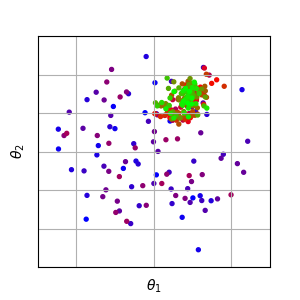
\includegraphics[width=\textwidth]{figures/mutation/simple_normal-100-10_none_normal-0.1_0-1.png}
        \caption{Normal with $\sigma=0.1$.}
        \label{subfig:mutation_normal_01}
    \end{subfigure}
    \begin{subfigure}[t]{0.24\textwidth}
        \centering
        \captionsetup{width=.9\textwidth}
        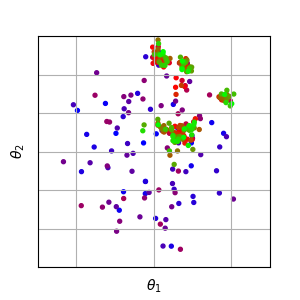
\includegraphics[width=\textwidth]{figures/mutation/simple_normal-100-10_none_onestep_0-1.png}
        \caption{Onestep.}
        \label{subfig:mutation_onestep_01}
    \end{subfigure}
    \begin{subfigure}[t]{0.24\textwidth}
        \centering
        \captionsetup{width=.9\textwidth}
        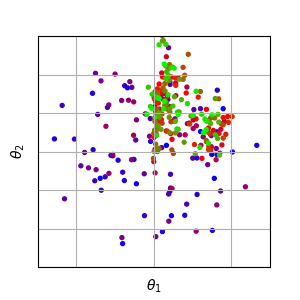
\includegraphics[width=\textwidth]{figures/mutation/simple_normal-100-10_none_nstep_0-1.png}
        \caption{NStep.}
        \label{subfig:mutation_nstep_01}
    \end{subfigure}
    
    \begin{subfigure}[t]{0.24\textwidth}
        \centering
        \captionsetup{width=.9\textwidth}
        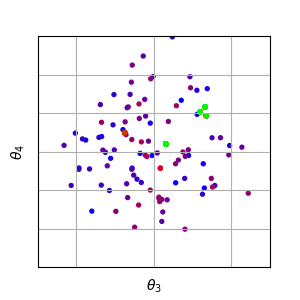
\includegraphics[width=\textwidth]{figures/recombination/simple_normal-100-10_2-3.png}
        \caption{None.}
        \label{subfig:mutation_none_23}
    \end{subfigure}
    \begin{subfigure}[t]{0.24\textwidth}
        \centering
        \captionsetup{width=.9\textwidth}
        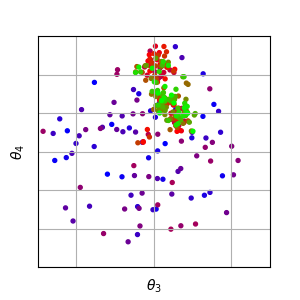
\includegraphics[width=\textwidth]{figures/mutation/simple_normal-100-10_none_normal-0.1_2-3.png}
        \caption{Normal with $\sigma=0.1$.}
        \label{subfig:mutation_normal_23}
    \end{subfigure}
    \begin{subfigure}[t]{0.24\textwidth}
        \centering
        \captionsetup{width=.9\textwidth}
        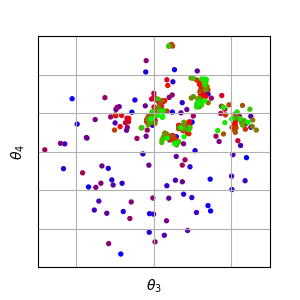
\includegraphics[width=\textwidth]{figures/mutation/simple_normal-100-10_none_onestep_2-3.png}
        \caption{OneStep.}
        \label{subfig:mutation_onestep_23}
    \end{subfigure}
    \begin{subfigure}[t]{0.24\textwidth}
        \centering
        \captionsetup{width=.9\textwidth}
        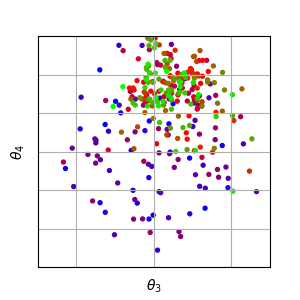
\includegraphics[width=\textwidth]{figures/mutation/simple_normal-100-10_none_nstep_2-3.png}
        \caption{NStep.}
        \label{subfig:mutation_nstep_23}
    \end{subfigure}
    \caption{Evolution of the simple player with a population size of $100$ and $10$ games per tournament for $20$ generations with different mutation methods. The color range of the plots goes from blue to green, thus a green area indicate many chromosomes.}
    \label{fig:mutation_method_simple}
\end{figure}
From figures \ref{subfig:mutation_none_01} and \ref{subfig:mutation_none_23} none mutation does not explore the search space. However, the normal mutation in figures \ref{subfig:mutation_normal_01} and \ref{subfig:mutation_normal_23} explores the space and converges towards one optimal solution. The OneStep mutation method shown in figures \ref{subfig:mutation_onestep_01} and \ref{subfig:mutation_onestep_23} seems to converges towards multiple optimal solution, thereby doing a better search than normal mutation. It would seem that the mutation method NStep shown in figures \ref{subfig:mutation_nstep_01} and \ref{subfig:mutation_nstep_23} has most diversity, and will therefore not converges to a local maximum but more likely a global. In figure \ref{subfig:evolution_simple_recomb_mutation} the different EA combinations from figure \ref{fig:recombination_method_simple} and \ref{fig:mutation_method_simple} are compared and perform similarly for the $20$ generations.

Based on figures \ref{fig:recombination_method_simple} and \ref{fig:mutation_method_simple} the simple player is evolved with blend recombination with $\alpha=0.5$ and NStep mutation. The different selection methods are evaluated in figure \ref{subfig:evolution_simple_comb} and a combination of normal selection, no recombination and no mutation is added for comparison.

\begin{figure}[t]
    \centering
    \begin{subfigure}[t]{0.49\textwidth}
        \centering
        \captionsetup{width=.9\textwidth}
        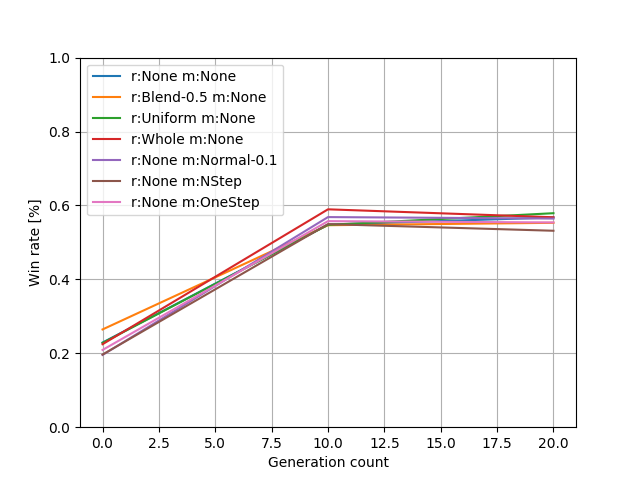
\includegraphics[width=\textwidth]{figures/simple/simple_recombs_mutations.png}
        \caption{Evolution of the simple player with different recombination and mutation methods.}
        \label{subfig:evolution_simple_recomb_mutation}
    \end{subfigure}
    \begin{subfigure}[t]{0.49\textwidth}
        \centering
        \captionsetup{width=.9\textwidth}
        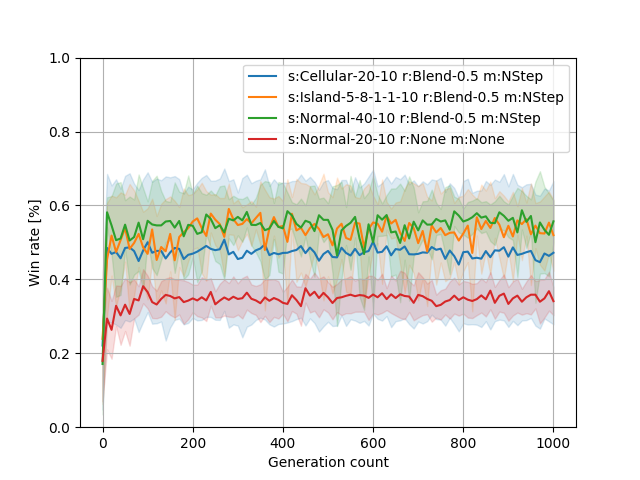
\includegraphics[width=\textwidth]{figures/simple/eval_simple.png}
        \caption{Evolution of the simple player with different selection methods.}
        \label{subfig:evolution_simple_comb}
    \end{subfigure}
    \caption{Evolution of the simple player with different combinations of EA components. Every $10$'th generation is evaluated against $3$ random players for $100$ games.}
    \label{fig:}
\end{figure}

In figure \ref{subfig:evolution_simple_comb} the different selection types perform similarly, however, the cellular selection has a slightly higher standard deviation. The best chromosome in the final population in the EA combination \texttt{s:Cellular-20-10 r:Blend-0.5 m:NStep} is found and used for evaluation of the simple player in section \ref{sec:results}.

\subsection{Evolution of the Advanced Player}
To find a good chromosome to the advanced player the different recombination and mutation methods are examined in figure \ref{fig:recomb_mutation_advanced}. The methods are evolved for $200$ generations with normal selection with a population size of $100$ and $10$ games per tournament, and each chromosome in the populations is evaluated against random players for $100$ games.  
\begin{figure}[t]
    \centering
    \begin{subfigure}[t]{0.49\textwidth}
        \centering
        \captionsetup{width=.9\textwidth}
        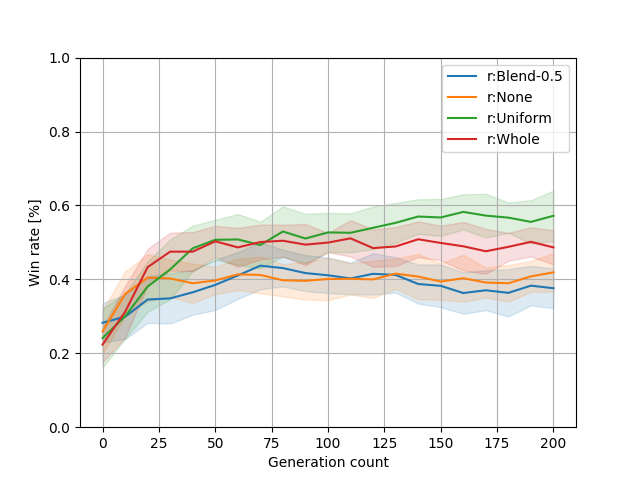
\includegraphics[width=\textwidth]{figures/recombination/eval_recombination_methods.png}
        \caption{Evolution of different recombination methods.}
        \label{subfig:recombs_advanced}
    \end{subfigure}
    \begin{subfigure}[t]{0.49\textwidth}
        \centering
        \captionsetup{width=.9\textwidth}
        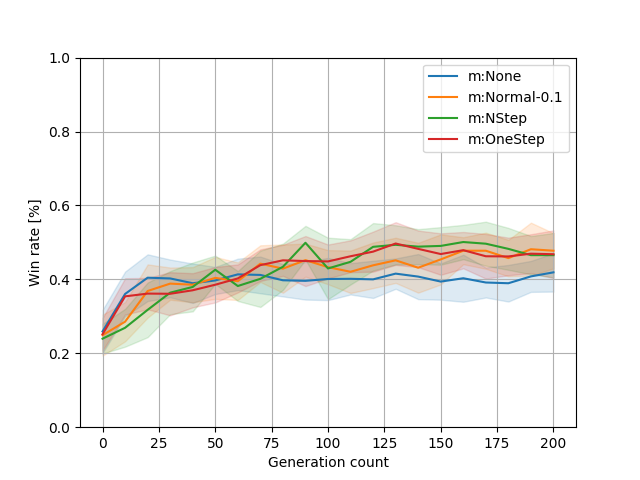
\includegraphics[width=\textwidth]{figures/mutation/eval_mutation_methods.png}
        \caption{Evolution of different mutation methods.}
        \label{subfig:mutations_advanced}
    \end{subfigure}
    \caption{Evolution of different recombination and mutation methods with normal selection and no mutation for $200$ generations of the advanced player. Every $10$'th generation is evaluated against $3$ random players for $100$ games.}
    \label{fig:recomb_mutation_advanced}
\end{figure}

From figure \ref{subfig:recombs_advanced}, the uniform recombination has the highest mean and standard deviation after $200$ generations against random players. Thus, the uniform recombination seems like a good hyperparameter. From figure \ref{subfig:mutations_advanced}, the different mutations seem to perform somewhat equally. However, none mutation underperforms as expected.

Based on figures \ref{subfig:recombs_advanced} and \ref{subfig:mutations_advanced}, the recombination method uniform and mutation method normal with $\sigma=0.1$ are used for evolving the advanced player. The evolution of the advanced player is shown in figure \ref{subfig:evolution_advanced_comb} with different EA combinations. A EA combination of normal selection, no recombination and no mutation is added for comparison. Every $10$'th population is evaluated against $3$ random players in $100$ games. Figure \ref{subfig:evolution_advanced_comb} shows that the best performing combination is \texttt{s:Normal-100-10 r:Whole m:Normal-0.1} that performs slightly better than \texttt{s:Cellular-100-10 r:Whole m:Normal-0.1} and \texttt{s:Normal-100-10 r:Uniform m:Normal-0.1}, thus its best chromosome of its final population is used for evaluation of the advanced player in section \ref{sec:results}.

\subsection{Evolution of the Full Player}
Based on the experience from the simple and advanced player the EA combination shown in figure \ref{subfig:evolution_full_comb} are explored.
\begin{figure}[t]
    \centering
    \begin{subfigure}[t]{0.49\textwidth}
        \centering
        \captionsetup{width=.9\textwidth}
        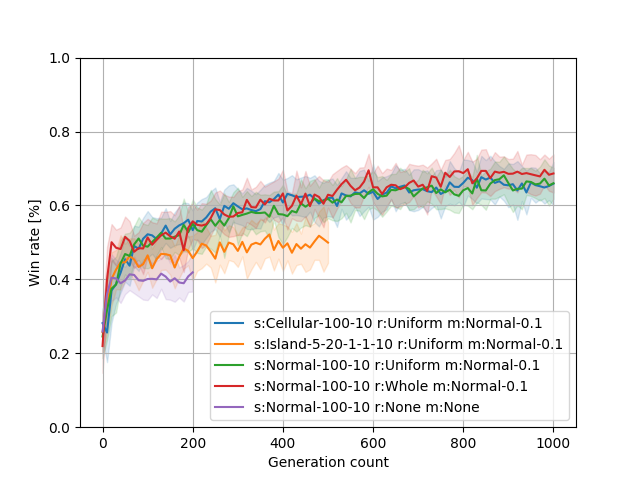
\includegraphics[width=\textwidth]{figures/advanced/advanced_combination.png}
        \caption{The advanced player}
        \label{subfig:evolution_advanced_comb}
    \end{subfigure}
    \begin{subfigure}[t]{0.49\textwidth}
        \centering
        \captionsetup{width=.9\textwidth}
        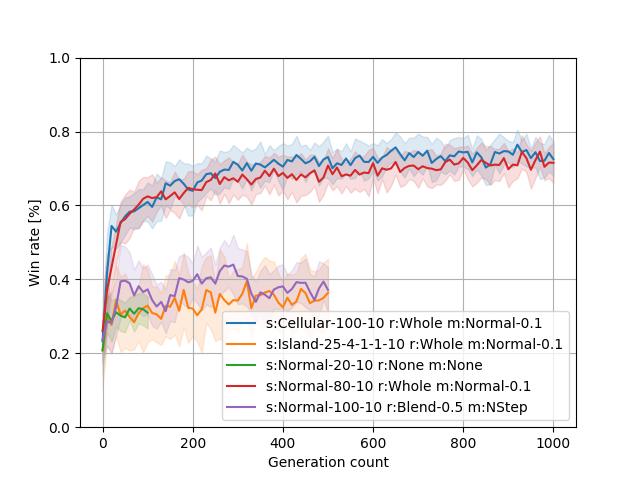
\includegraphics[width=\textwidth]{figures/full/ann_combinations.png}
        \caption{The full player}
        \label{subfig:evolution_full_comb}
    \end{subfigure}
    \caption{Evolution of the advanced and full player with different combination of EA components. Each chromosome in each generation is evaluated against $3$ random players for $100$ games.}
    \label{fig:evolution_advanced_full}
\end{figure}

In figure \ref{subfig:evolution_full_comb}, it can be seen that after $100$ generation the combination \texttt{s:Normal-20-10 r:None m:None} does not performs as good as the other combination and is discarded. After $500$ generations the best performing combinations are \texttt{s:Cellular-100-10 r:Whole m:Normal-0.1} and \texttt{s:Normal-80-10 r:Whole m:Normal-0.1}, these combination are evolved for $500$ generation more. The combination \texttt{s:Cellular-100-10 r:Whole m:Normal-0.1} performs slightly better than \texttt{s:Normal-80-10 r:Whole m:Normal-0.1} after $1000$ generations, thus the best chromosome from the last population is used for the full player in the evaluation in section \ref{sec:results}.

\subsection{Hyperparameters Tuning of Evolutionary Algorithms}
In this paper many different combinations of EA components have been investigated, however, it could be that the best tuning of parameters is still out there. Therefore, a random search method for finding good indications of parameters could be implemented. A random search would then run for a fixed number of iterations and evaluated randomly put together parameters for a fixed number of games against random players. However, in this paper it was not deemed necessary.

\subsection{Advanced vs. Full}
The two implemented artificial neural networks are quite similar, but the advanced has only 948 parameters and the full has 23800 parameters. However, the advanced score against random players is $91.6\ \%$ and the full is $92.5\ \%$, and the full has $25$ times more parameters. However, notice that the gap between the advanced and full player is at $0.9$ against random and $6.7$ against smart players in table \ref{tab:player_eval}. The full player wins $56.9\ \%$ against the advanced player, this also indicates the difference between the two players is larger than $0.9$. Furthermore, the prediction time for choosing a token is for the full $0.000432$ seconds and the advanced $0.000172$ seconds. This must all be taken into account when developing an artificial neural network because the computation capacity and time becomes a factor with large networks. Thus, if a complex task is at hand a large network might be needed. However, if a smaller network can do the job it should be considered. 

\subsection{Weight Initialization of the Neural Network} \label{subsec:weight_init}
The weight initialization of the two neural networks is sampled from a normal distribution, however, in \cite{tanh_activations} they show good results with initializing the weights with a standard deviation of $\sqrt{1/N}$ when using Tanh as the activation function. This was added to the full player by introducing a bias term of $\sqrt{1/N}$ that is multiplied with the hidden layer outputs. If it were to be added to the advanced player it might help boost performance.

\section{Conclusion} \label{sec:conclusion}
This paper has explored methods for making an artificial ludo player by the use of an artificial neural network that was optimized by evolutionary algorithms. For the evolutionary algorithms different selection and reproduction methods have been used.

In total three players have been evolved using different evolutionary methods. One with domain knowledge, the simple player, and two without domain knowledge, the advanced and full player. However, the two without domain knowledge performs better than the one with domain knowledge.

The simple player wins $80.1\ \%$ against random players with two instances of each player, the advanced player wins $91.6\ \%$ and the full player wins $92.5\ \%$.

\section{Acknowledgement} \label{sec:acknowledgement}

Thanks to Mikkel Larsen for the use of his Q-learning player and help throughout this project. Furthermore, thanks to Rasmus Haugaard for the python version of the ludo game.

\begin{thebibliography}{}
% \bibitem{code:github}
% Slettemark-Nielsen, M. E.:
% \url{https://github.com/Masle16/ludo_ai2}
% (accessed 25 May 2020)

\bibitem{ec:springer}
Eiben, A. E. and Smith, James E.:
Introduction to Evolutionary Computing.
Springer Publishing Company, Incorporated.
978-3-662-44874-8 (2015)

\bibitem{ludo_game}
Haugaard, R.:
\url{https://github.com/RasmusHaugaard/pyludo}:
(accessed 20 May 2020)

\bibitem{z_test}
Binomial test, Wikipedia:
\url{https://en.wikipedia.org/wiki/Binomial_test}:
(accessed 18 May 2020)

\bibitem{mikkel}
Larsen, M.:
\url{https://github.com/mikkellars/pyludo}:
(accessed 21 May 2020)

\bibitem{tanh_activations}
Glorot, X. and Bengio, Y.:
Understanding the difficulty of training deep feedforward neural networks:
Proceedings of the thirteenth international conference on artificial intelligence and statistics:
pages 249-256:
(2010)

\end{thebibliography}

\end{document}
